% =============================================================================
% Indirect reciprocity with inertial reputation updating
% Slides for a discussion with Christian Hilbe (November 2026)
%
% Theme: metropolis (16:9). Compile with pdfLaTeX + BibTeX
% (latexmk -pdf IR_Hilbe_slides.tex). On Overleaf, compile as usual.
% Figures are searched in figures/ and, inside the repository, in ../Manuscript_doc/.
% This file was generated from build/deck_spec.py; it can be edited directly.
% =============================================================================
\documentclass[aspectratio=169,10pt,t,xcolor=table]{beamer}
\usetheme[progressbar=none,numbering=counter,block=fill,sectionpage=none]{metropolis}
\usefonttheme[onlymath]{serif}
\usepackage{appendixnumberbeamer}
\usepackage{amsmath,amssymb,mathrsfs,bm,booktabs,array}
\usepackage{tikz}
\usetikzlibrary{arrows.meta,positioning,calc}
\usepackage[authoryear,round]{natbib}
\graphicspath{{figures/}{../Manuscript_doc/}}

% ----------------------------------------------------------------- colors
\definecolor{ink}{HTML}{23373B}
\definecolor{accent}{HTML}{EB811B}
\definecolor{blueacc}{HTML}{2F6E9E}
\definecolor{muted}{HTML}{6B7B80}
\definecolor{cardbg}{HTML}{EEF2F3}
\definecolor{goodimg}{HTML}{3B7DB8}
\definecolor{badimg}{HTML}{E58A9A}
\setbeamercolor{background canvas}{bg=white}
\setbeamercolor{normal text}{fg=ink,bg=white}
\setbeamercolor{frametitle}{bg=white,fg=ink}
\setbeamercolor{alerted text}{fg=accent}
\setbeamercolor{footline}{fg=muted}
\setbeamercolor{block title}{bg=cardbg,fg=ink}
\setbeamercolor{block body}{bg=cardbg,fg=ink}
\setbeamercolor{block title alerted}{bg=accent!16,fg=accent!75!black}
\setbeamercolor{block body alerted}{bg=accent!16,fg=ink}
\setbeamercolor{block title example}{bg=blueacc!13,fg=blueacc!85!black}
\setbeamercolor{block body example}{bg=blueacc!13,fg=ink}
\setbeamerfont{frametitle}{size=\large,series=\bfseries}
\setbeamerfont{block title}{size=\small,series=\bfseries}
\setbeamertemplate{itemize item}{\color{accent}\raisebox{1pt}{\scalebox{0.8}{$\blacktriangleright$}}}
\setlength{\leftmargini}{1.1em}

% ----------------------------------------------------------------- helpers
% Source line at the bottom left of a slide
\newcommand{\source}[1]{%
  \begin{tikzpicture}[remember picture,overlay]
    \node[anchor=south west,font=\tiny,text=muted,text width=13.2cm,align=left,inner sep=0pt]
      at ([xshift=0.48cm,yshift=0.22cm]current page.south west) {#1};
  \end{tikzpicture}}
% Storyline tag at the top right of a slide
\newcommand{\slidetag}[2]{%
  \begin{tikzpicture}[remember picture,overlay]
    \node[anchor=north east,fill=#1!15,text=#1!80!black,font=\scriptsize\bfseries,
          rounded corners=2pt,inner xsep=5pt,inner ysep=3pt]
      at ([xshift=-0.42cm,yshift=-0.32cm]current page.north east) {#2};
  \end{tikzpicture}}
% Key message box
\newcommand{\takeaway}[1]{\par\vspace{3pt}\noindent
  \begin{tikzpicture}
    \node[fill=accent!13,rounded corners=3pt,text width=\dimexpr\linewidth-12pt\relax,
          inner sep=6pt,align=left,font=\small]{#1};
  \end{tikzpicture}\par\vspace{2pt}}
% Display equation with optional lead text
\newcommand{\eqlead}[1]{{\small #1\par}\vspace{-1pt}}
\newcommand{\eqline}[2]{{\centering #1\mbox{$\displaystyle #2$}\par}\vspace{2pt}}
% Figure caption and small notes
\newcommand{\figcap}[1]{{\scriptsize\color{muted}#1\par}}
\newcommand{\smallnote}[1]{{\scriptsize\color{muted}\itshape #1\par}}
\newenvironment{cardlist}{\begin{itemize}\setlength{\itemsep}{1pt}\small}{\end{itemize}}

% ----------------------------------------------------------------- title data
\title{Indirect reciprocity with inertial reputation updating}
\author{Wenqiang Zhu}
\date{}
\begin{document}

% ---------------------------------------------------------------- slide 1
{\setbeamercolor{background canvas}{bg=ink}
\begin{frame}[plain,noframenumbering]
\vspace*{1.55cm}
{\color{white}\fontsize{21}{26}\selectfont\bfseries Indirect reciprocity with inertial reputation updating\par}
\vspace{0.35cm}
{\color{accent}\large How reputations accumulate and express behavioral evidence\par}
\vspace{1.1cm}
{\color{white}\normalsize\bfseries Wenqiang Zhu\par}
\vspace{2pt}
{\color{white!72!ink}\small School of Artificial Intelligence, Beihang University\par}
\vspace{0.45cm}
{\color{white!72!ink}\small Discussion with Christian Hilbe · November 2026\par}
\end{frame}}

% ---------------------------------------------------------------- slide 2
\begin{frame}{Overview}\relax
\vspace{6pt}\begin{tabular}{@{}m{0.8cm}m{0.85\linewidth}@{}}
\tikz\node[circle,fill=accent,text=white,font=\small\bfseries,minimum size=0.62cm,inner sep=0pt]{1}; & \textbf{Motivation and research gap}\newline{\small\color{muted}Two candidate storylines (Introduction V1 and V2)}\\[7pt]
\tikz\node[circle,fill=accent,text=white,font=\small\bfseries,minimum size=0.62cm,inner sep=0pt]{2}; & \textbf{Model and methods}\newline{\small\color{muted}Inertial records, stationary reputation map, population theory, invasion analysis}\\[7pt]
\tikz\node[circle,fill=accent,text=white,font=\small\bfseries,minimum size=0.62cm,inner sep=0pt]{3}; & \textbf{Results}\newline{\small\color{muted}Main-text Figs. 2–5}\\[7pt]
\tikz\node[circle,fill=accent,text=white,font=\small\bfseries,minimum size=0.62cm,inner sep=0pt]{4}; & \textbf{Conclusion}\newline{\small\color{muted}Answers to the research gap and points for discussion}\\[7pt]
\tikz\node[circle,fill=accent,text=white,font=\small\bfseries,minimum size=0.62cm,inner sep=0pt]{5}; & \textbf{Supplementary results}\newline{\small\color{muted}Extended Data and analytical results (backup)}\\[7pt]
\end{tabular}
\end{frame}

% ---------------------------------------------------------------- slide 3
\section{Motivation and research gap}
{\setbeamercolor{background canvas}{bg=ink}
\begin{frame}[plain,noframenumbering]
\vspace*{2.0cm}
{\color{accent}\fontsize{40}{44}\selectfont\bfseries 1\par}
\vspace{0.3cm}
{\color{white}\fontsize{22}{26}\selectfont\bfseries Motivation and research gap\par}
\end{frame}}

% ---------------------------------------------------------------- slide 4
\begin{frame}{Two candidate storylines}\relax
\begin{columns}[T,onlytextwidth]
\begin{column}{0.485\textwidth}
\begin{exampleblock}{Storyline A · Introduction V1}
\begin{cardlist}
  \item Start from the failure of classical norms under private assessment
  \item Identify overwrite updating as a root cause of the fragility
  \item End with two explicit open questions about evidence
\end{cardlist}
\end{exampleblock}
\end{column}
\hfill
\begin{column}{0.485\textwidth}
\begin{alertblock}{Storyline B · Introduction V2}
\begin{cardlist}
  \item Start from reputation as a currency of social life
  \item Ask how a reputation system should integrate evidence over time
  \item Motivate directional inertia by human evaluation and institutions
\end{cardlist}
\end{alertblock}
\end{column}
\end{columns}
\vspace{4pt}
{\small {\color{muted}Both storylines lead to the same framework and the same results. The following slides present each line in turn, then compare them.}\par}\vspace{3pt}
\end{frame}

% ---------------------------------------------------------------- slide 5
\begin{frame}{Classical norms need reputations that are shared}\relax
\slidetag{blueacc}{Storyline A · Intro V1}
\source{Nowak \& Sigmund 1998, 2005; Ohtsuki \& Iwasa 2004, 2006; Hilbe et al. 2018; Fujimoto \& Ohtsuki 2022, 2023}
{\normalsize
\begin{itemize}
  \item Helping others raises one's standing and the chance of being helped by third parties (indirect reciprocity).
  \item The leading-eight norms stabilize cooperation when reputations are public, even with occasional errors.
  \item Under private, noisy assessment, observers hold different views of the same person, and most leading-eight norms fail.
\end{itemize}}
\par\vspace{4pt}{\centering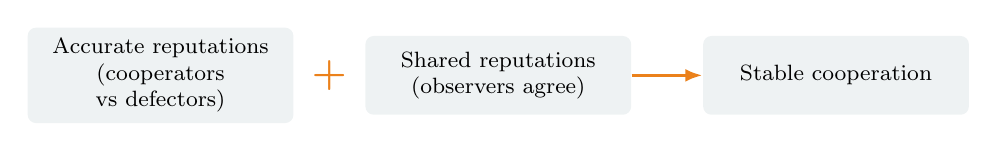
\begin{tikzpicture}[box/.style={fill=cardbg,rounded corners=3pt,align=center,font=\footnotesize,minimum height=1.0cm,inner sep=4pt,text width=\dimexpr(\linewidth-2cm)/3-8pt\relax}]
  \node[box] (n0) {Accurate reputations\\(cooperators vs defectors)};
  \node[box, right=0.90cm of n0] (n1) {Shared reputations\\(observers agree)};
  \node[box, right=0.90cm of n1] (n2) {Stable cooperation};
  \node[font=\Large\bfseries,text=accent] at ($(n0.east)!0.5!(n1.west)$) {+};
  \draw[-{Latex[length=2.2mm]},very thick,accent] (n1.east) -- (n2.west);
\end{tikzpicture}\par}\vspace{4pt}
\takeaway{Central problem: under private assessment, reputations must remain both \textbf{accurate} and \textbf{shared}.}
\end{frame}

% ---------------------------------------------------------------- slide 6
\begin{frame}{Part of the fragility lies in how reputations are updated}\relax
\slidetag{blueacc}{Storyline A · Intro V1}
\source{Ohtsuki \& Iwasa 2004; Hilbe et al. 2018; Radzvilavicius et al. 2019; Okada 2020}
{\normalsize
\begin{itemize}
  \item In the standard binary framework, every new assessment replaces the previous image.
  \item A single error can reverse a reputation built over many interactions, and the next observation can reverse it again.
  \item Under private assessment these flips spread. Discriminators are condemned when observers disagree about the recipient.
\end{itemize}}
\par\vspace{2pt}{\centering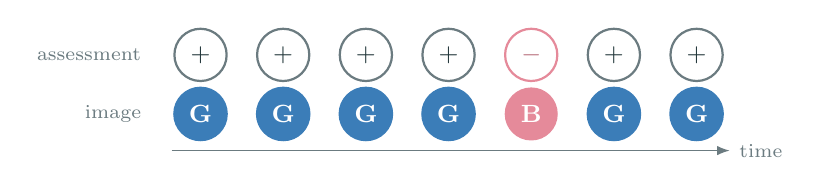
\begin{tikzpicture}[x=1.05cm,y=0.75cm]
  \node[anchor=east,font=\scriptsize,text=muted] at (-0.6,0) {assessment};
  \node[anchor=east,font=\scriptsize,text=muted] at (-0.6,-1) {image};
  \node[circle,draw=muted,thick,minimum size=0.55cm,font=\small\bfseries,text=ink] at (0,0) {$+$};
  \node[circle,fill=goodimg,minimum size=0.55cm,font=\small\bfseries,text=white] at (0,-1) {G};
  \node[circle,draw=muted,thick,minimum size=0.55cm,font=\small\bfseries,text=ink] at (1,0) {$+$};
  \node[circle,fill=goodimg,minimum size=0.55cm,font=\small\bfseries,text=white] at (1,-1) {G};
  \node[circle,draw=muted,thick,minimum size=0.55cm,font=\small\bfseries,text=ink] at (2,0) {$+$};
  \node[circle,fill=goodimg,minimum size=0.55cm,font=\small\bfseries,text=white] at (2,-1) {G};
  \node[circle,draw=muted,thick,minimum size=0.55cm,font=\small\bfseries,text=ink] at (3,0) {$+$};
  \node[circle,fill=goodimg,minimum size=0.55cm,font=\small\bfseries,text=white] at (3,-1) {G};
  \node[circle,draw=badimg,thick,minimum size=0.55cm,font=\small\bfseries,text=badimg!80!black] at (4,0) {$-$};
  \node[circle,fill=badimg,minimum size=0.55cm,font=\small\bfseries,text=white] at (4,-1) {B};
  \node[circle,draw=muted,thick,minimum size=0.55cm,font=\small\bfseries,text=ink] at (5,0) {$+$};
  \node[circle,fill=goodimg,minimum size=0.55cm,font=\small\bfseries,text=white] at (5,-1) {G};
  \node[circle,draw=muted,thick,minimum size=0.55cm,font=\small\bfseries,text=ink] at (6,0) {$+$};
  \node[circle,fill=goodimg,minimum size=0.55cm,font=\small\bfseries,text=white] at (6,-1) {G};
  \draw[-{Latex[length=1.6mm]},muted] (-0.35,-1.62) -- (6.40,-1.62) node[right,font=\scriptsize,text=muted] {time};
\end{tikzpicture}\par}\vspace{2pt}
\takeaway{Cooperation depends not only on \textbf{which norm} is used, but also on \textbf{how much evidence} is required before a judgment is revised.}
\end{frame}

% ---------------------------------------------------------------- slide 7
\begin{frame}{Existing remedies treat losing and regaining standing alike}\relax
\slidetag{blueacc}{Storyline A · Intro V1}
\source{Radzvilavicius et al. 2019, 2021; Kawakatsu et al. 2024; Murase \& Hilbe 2023, 2024; Tham et al. 2026; Schmid et al. 2021, 2023; Clark et al. 2020; Michel-Mata et al. 2024}
\begin{columns}[T,onlytextwidth]
\begin{column}{0.485\textwidth}
\begin{block}{Restore agreement}
\begin{cardlist}
  \item Public institutions
  \item Gossip
  \item Empathetic evaluation
  \item Opinion synchronization
\end{cardlist}
\end{block}
\end{column}
\hfill
\begin{column}{0.485\textwidth}
\begin{block}{Integrate more information}
\begin{cardlist}
  \item Generous or stochastic assessment
  \item Graded reputations, reasoning about errors
  \item Quantitative scores
  \item Aggregation of observations
\end{cardlist}
\end{block}
\end{column}
\end{columns}
\vspace{4pt}
{\small Using more than the latest observation helps but needs tolerance, and tolerance can also forgive deliberate defection. Loss and recovery of standing are governed by one score, threshold or window.\par}\vspace{3pt}
\begin{alertblock}{Open questions}
\begin{cardlist}
  \item Should losing and regaining standing require different amounts of evidence?
  \item How should accumulating but inconclusive evidence affect how a person is treated?
\end{cardlist}
\end{alertblock}
\end{frame}

% ---------------------------------------------------------------- slide 8
\begin{frame}{Societies separate an accumulating record from a verdict}\relax
\slidetag{blueacc}{Storyline A · Intro V1}
\source{Ostrom 1990; Cox et al. 2010; Tadelis 2016; Blumstein \& Nakamura 2009; Mende-Siedlecki et al. 2013; Slovic 1993; Siegel et al. 2018}
\begin{columns}[T,onlytextwidth]
\begin{column}{0.485\textwidth}
\begin{block}{Institutions}
\begin{cardlist}
  \item Graduated sanctions escalate with repeated violations
  \item Online markets summarize long feedback histories
  \item Criminal records stop signaling risk only after years
\end{cardlist}
\end{block}
\end{column}
\hfill
\begin{column}{0.485\textwidth}
\begin{block}{Impression formation}
\begin{cardlist}
  \item Impressions are updated as behavior unfolds
  \item The weight of new evidence depends on its diagnostic value
  \item Asymmetries run both ways: trust is lost faster, beliefs about bad people are volatile
\end{cardlist}
\end{block}
\end{column}
\end{columns}
\vspace{4pt}
\takeaway{Standing can persist while contrary evidence accumulates, and losing and regaining it need not require the same evidence.}
\end{frame}

% ---------------------------------------------------------------- slide 9
\begin{frame}{Private information makes reputations fragile}\relax
\slidetag{accent}{Storyline B · Intro V2}
\source{Milinski 2016; Nowak \& Sigmund 2005; Hilbe et al. 2018; Murase \& Hilbe 2024; Schmid et al. 2023; Michel-Mata et al. 2024}
\begin{columns}[T,onlytextwidth]
\begin{column}{0.56\textwidth}
{\normalsize
\begin{itemize}
  \item Reputation lets past behavior shape future opportunities, and social norms turn behavior into moral standing.
  \item Classical norms sustain cooperation when observers agree on each other's standing.
  \item In reality, information is noisy and privately interpreted, so observers disagree whether an action was justified.
  \item In binary models each assessment overwrites the image, so a single mistake can undo a long record.
\end{itemize}}
\end{column}
\hfill
\begin{column}{0.40\textwidth}
\begin{block}{Recent remedies}
\begin{cardlist}
  \item \textbf{Restore agreement:} institutions, gossip, empathy, opinion synchronization
  \item \textbf{Use more information:} generosity, graded reputations, reasoning about errors, quantitative scores, aggregation
\end{cardlist}
\end{block}
{\small {\color{muted}These approaches show that information beyond the latest observation can stabilize cooperation.}\par}\vspace{3pt}
\end{column}
\end{columns}
\end{frame}

% ---------------------------------------------------------------- slide 10
\begin{frame}{Gap: how should reputations integrate evidence over time?}\relax
\slidetag{accent}{Storyline B · Intro V2}
\source{Schmid et al. 2023; Michel-Mata et al. 2024; Yamamoto et al. 2025; Siegel et al. 2018; Ostrom 1990; Blumstein \& Nakamura 2009}
\begin{columns}[T,onlytextwidth]
\begin{column}{0.52\textwidth}
{\normalsize
\begin{itemize}
  \item Accumulating information is not the same as using more of it.
  \item A good reputation may persist while contrary evidence accumulates, and recovery may follow a different process.
  \item Existing approaches treat losing and regaining standing as one process, with one score, threshold or window.
\end{itemize}}
\end{column}
\hfill
\begin{column}{0.44\textwidth}
\begin{block}{Human evaluation is directional}
\begin{cardlist}
  \item Impressions are revised over sequences of behavior
  \item Good and bad individuals are updated asymmetrically
  \item Graduated sanctions escalate with repeated violations
  \item Restoring standing after a criminal record takes years
\end{cardlist}
\end{block}
\end{column}
\end{columns}
\vspace{2pt}
\takeaway{Standing should have inertia, and the inertia of losing standing may differ from that of regaining it.}
\end{frame}

% ---------------------------------------------------------------- slide 11
\begin{frame}{The two storylines at a glance}\relax
{\small
\begin{tabular}{@{}>{\raggedright\arraybackslash}p{\dimexpr0.180\linewidth-2\tabcolsep\relax}>{\raggedright\arraybackslash}p{\dimexpr0.410\linewidth-2\tabcolsep\relax}>{\raggedright\arraybackslash}p{\dimexpr0.410\linewidth-2\tabcolsep\relax}@{}}
\toprule
\rowcolor{cardbg} & \textbf{Storyline A (Introduction V1)} & \textbf{Storyline B (Introduction V2)} \\
\midrule
\textbf{Opening} & Leading-eight norms fail under private assessment & Reputation as a currency of social life \\
\textbf{Central problem} & Reputations must be accurate and shared & How should evidence be integrated over time? \\
\textbf{Diagnosis} & Overwrite updating triggers disagreement cascades & Loss and recovery are treated as one process \\
\textbf{Gap} & Two explicit questions: evidence asymmetry and the role of inconclusive evidence & Directional inertia, motivated by human evaluation and institutions \\
\textbf{Tone} & Problem-driven, close to the private-assessment literature & Conceptual, aimed at a broad readership \\
\bottomrule
\end{tabular}}\par\vspace{3pt}
\end{frame}

% ---------------------------------------------------------------- slide 12
\begin{frame}{This work: separate accumulation from interpretation of evidence}\relax
\begin{columns}[T,onlytextwidth]
\begin{column}{0.46\textwidth}
\begin{exampleblock}{Evidence accumulation}
{\small Depths $k_1$, $k_2$ determine how much consistent evidence changes an established reputation.\par}
\end{exampleblock}
\begin{alertblock}{Evidence interpretation}
{\small Strengths $\alpha$, $\beta$ determine how strongly incomplete evidence already affects treatment.\par}
\end{alertblock}
\end{column}
\hfill
\begin{column}{0.50\textwidth}
{\normalsize \textbf{Main findings}\par}\vspace{3pt}
{\normalsize
\begin{itemize}
  \item The \textbf{allocation} of inertia between losing and regaining standing determines whether private reputations are accurate and shared.
  \item Compact, norm-specific architectures make cooperation \textbf{stable and accessible}. Allocation matters more than amount.
  \item Tolerance \textbf{shelters occasional defectors}. Giving warning states partial consequences restores deterrence.
\end{itemize}}
\end{column}
\end{columns}
\end{frame}

% ---------------------------------------------------------------- slide 13
\section{Model and methods}
{\setbeamercolor{background canvas}{bg=ink}
\begin{frame}[plain,noframenumbering]
\vspace*{2.0cm}
{\color{accent}\fontsize{40}{44}\selectfont\bfseries 2\par}
\vspace{0.3cm}
{\color{white}\fontsize{22}{26}\selectfont\bfseries Model and methods\par}
\end{frame}}

% ---------------------------------------------------------------- slide 14
\begin{frame}{Donation game with private assessment}\relax
\source{Reference parameters: $b/c=5$, $e_1=e_2=0.02$}
\begin{columns}[T,onlytextwidth]
\begin{column}{0.60\textwidth}
{\small
\begin{itemize}
  \item A donor pays $c$ and the recipient gains $b>c$. Strategies: ALLC, ALLD and DISC (helps recipients it regards as good).
  \item A random observer judges the action with \textbf{its own} image of the recipient (private assessment).
  \item Errors: failed cooperation ($e_1$) and reversed assessment ($e_2$).
\end{itemize}}
\end{column}
\hfill
\begin{column}{0.36\textwidth}
{\footnotesize
\begin{tabular}{@{}>{\raggedright\arraybackslash}p{\dimexpr0.700\linewidth-2\tabcolsep\relax}>{\raggedright\arraybackslash}p{\dimexpr0.150\linewidth-2\tabcolsep\relax}>{\raggedright\arraybackslash}p{\dimexpr0.150\linewidth-2\tabcolsep\relax}@{}}
\toprule
\rowcolor{cardbg}\textbf{Norm} & \textbf{$p$} & \textbf{$q$} \\
\midrule
\textbf{Scoring (SC)} & 1 & 0 \\
\textbf{Shunning (SH)} & 0 & 0 \\
\textbf{Stern Judging (SJ)} & 0 & 1 \\
\textbf{Simple Standing (SS)} & 1 & 1 \\
\bottomrule
\end{tabular}}\par\vspace{3pt}
{\footnotesize {\color{muted}$p$, $q$: probability that C or D towards a recipient regarded as bad is assessed as good. C towards a good recipient is good, D is bad.}\par}\vspace{3pt}
\end{column}
\end{columns}
\vspace{2pt}
\eqlead{Positive recorded assessment, given intended action and the observer's image of the recipient:}
\eqline{\small}{P^{+}_{\mathrm{C|G}}=\varepsilon,\quad P^{+}_{\mathrm{D|G}}=e_2,\quad P^{+}_{\mathrm{D|B}}=e_2+(1-2e_2)\,q}
\eqline{\small}{P^{+}_{\mathrm{C|B}}=e_2+(1-2e_2)\bigl[(1-e_1)\,p+e_1\,q\bigr],\quad \varepsilon=(1-e_1)(1-e_2)+e_1e_2}
\end{frame}

% ---------------------------------------------------------------- slide 15
\begin{frame}{Inertial reputation updating}\relax
\begin{columns}[T,onlytextwidth]
\begin{column}{0.44\textwidth}
{\centering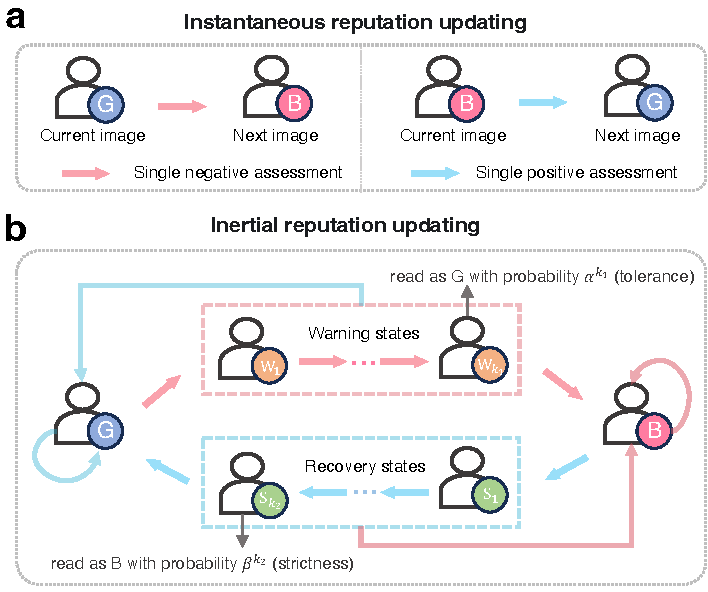
\includegraphics[width=\linewidth,height=0.68\textheight,keepaspectratio]{Fig1_model}\par}
\vspace{3pt}\figcap{\textbf{Fig. 1} | \textbf{a}, instantaneous updating. \textbf{b}, inertial updating with warning and recovery paths. An assessment in the opposite direction returns the record to the established state.}
\end{column}
\hfill
\begin{column}{0.52\textwidth}
{\small
\begin{itemize}
  \item Tolerance depth $k_1$: warning states $\mathrm{W}_m$. Strictness depth $k_2$: recovery states $\mathrm{S}_n$.
  \item Loss needs $k_1+1$ consecutive negative assessments, recovery $k_2+1$ positive ones.
\end{itemize}}
\eqlead{A consulted record is interpreted as good with probability}
\eqline{\small}{\sigma(\mathrm{G})=1,\qquad \sigma(\mathrm{W}_m)=\alpha^m}
\eqline{\small}{\sigma(\mathrm{B})=0,\qquad \sigma(\mathrm{S}_n)=1-\beta^n}
\begin{block}{Compared settings ($\alpha=\beta=1$)}
\begin{cardlist}
  \item No inertia $(0,0)$ and one-step $(1,1)$
  \item Selected: SC $(2,0)$, SH $(3,0)$, SJ $(4,3)$, SS $(1,2)$
\end{cardlist}
\end{block}
\end{column}
\end{columns}
\end{frame}

% ---------------------------------------------------------------- slide 16
\begin{frame}{Two levels of analysis}\relax
\par\vspace{4pt}{\centering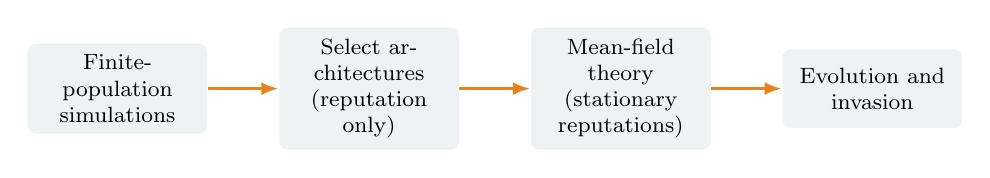
\begin{tikzpicture}[box/.style={fill=cardbg,rounded corners=3pt,align=center,font=\footnotesize,minimum height=1.0cm,inner sep=4pt,text width=\dimexpr(\linewidth-3cm)/4-8pt\relax}]
  \node[box] (n0) {Finite-population\\simulations};
  \node[box, right=0.90cm of n0] (n1) {Select architectures\\(reputation only)};
  \node[box, right=0.90cm of n1] (n2) {Mean-field theory\\(stationary reputations)};
  \node[box, right=0.90cm of n2] (n3) {Evolution and\\invasion};
  \draw[-{Latex[length=2.2mm]},very thick,accent] (n0.east) -- (n1.west);
  \draw[-{Latex[length=2.2mm]},very thick,accent] (n1.east) -- (n2.west);
  \draw[-{Latex[length=2.2mm]},very thick,accent] (n2.east) -- (n3.west);
\end{tikzpicture}\par}\vspace{4pt}
\begin{columns}[T,onlytextwidth]
\begin{column}{0.485\textwidth}
\begin{block}{Reputation formation (Fig. 2)}
\begin{cardlist}
  \item $N=150$, equal numbers of ALLC, ALLD and DISC
  \item Every DISC keeps a record of everyone; no closure
  \item 30 replicates and a drift check for the selection
\end{cardlist}
\end{block}
\end{column}
\hfill
\begin{column}{0.485\textwidth}
\begin{block}{Evolutionary analysis (Figs. 3–5)}
\begin{cardlist}
  \item Reputations equilibrate faster than strategies
  \item Replicator dynamics from 512 area-uniform initial compositions
  \item Local invasion by rare ALLC, ALLD and O-DISC mutants
\end{cardlist}
\end{block}
\end{column}
\end{columns}
\vspace{4pt}
\end{frame}

% ---------------------------------------------------------------- slide 17
\begin{frame}{Measuring recognition and agreement}\relax
{\normalsize
\begin{itemize}
  \item $g_I$: probability that a DISC observer regards a type-$I$ individual as good.
  \item $d_I$: probability that two DISC observers disagree about the same type-$I$ individual.
\end{itemize}}
\eqline{\normalsize}{\Delta g=\frac{g_{\mathrm{DISC}}+g_{\mathrm{ALLC}}}{2}-g_{\mathrm{ALLD}},\qquad \bar d=\sum_I\frac{n_I}{N}\,d_I}
{\normalsize
\begin{itemize}
  \item \textbf{Selection rule:} among allocations with $\Delta g\geq0.8$ and $\bar d\leq0.1$, take the smallest total depth $K=k_1+k_2$.
  \item \textbf{Selected:} SC $(2,0)$, SH $(3,0)$, SJ $(4,3)$, SS $(1,2)$, chosen without reference to evolutionary outcomes.
\end{itemize}}
\takeaway{Agreement alone is not enough: observers can agree that everyone is bad.}
\end{frame}

% ---------------------------------------------------------------- slide 18
\begin{frame}{The stationary reputation map}\relax
{\small A record with independent assessments, positive with probability $u$ ($v=1-u$), is a Markov chain $T(u)=uT^{+}+vT^{-}$.\par}\vspace{3pt}
\eqlead{\textbf{1} Path states are entered only from their predecessor:}
\eqline{\small}{\pi_{\mathrm{W}_m}=v^m\,\pi_{\mathrm{G}},\qquad \pi_{\mathrm{S}_n}=u^n\,\pi_{\mathrm{B}}}
\eqlead{\textbf{2} Flux balance between good and bad standing:}
\eqline{\small}{v^{k_1+1}\,\pi_{\mathrm{G}}=u^{k_2+1}\,\pi_{\mathrm{B}}}
\eqlead{\textbf{3} Normalization:}
\eqline{\small}{\pi_{\mathrm{G}}=\frac{u^{k_2+1}}{Z(u)},\qquad \pi_{\mathrm{B}}=\frac{v^{k_1+1}}{Z(u)},\qquad Z(u)=v^{k_1}+u^{k_2}-v^{k_1}u^{k_2}}
\eqlead{\textbf{4} Reputation map (stationary probability of being regarded as good):}
\eqline{\small}{\mathscr{R}(u)=\sum_{\ell}\pi_\ell(u)\,\sigma(\ell)=\frac{u^{k_2+1}\sum_{m=0}^{k_1}(\alpha v)^m+v^{k_1+1}\sum_{n=1}^{k_2}u^n(1-\beta^n)}{v^{k_1}+u^{k_2}-v^{k_1}u^{k_2}}}
\end{frame}

% ---------------------------------------------------------------- slide 19
\begin{frame}{Properties of the reputation map}\relax
\begin{columns}[T,onlytextwidth]
\begin{column}{0.55\textwidth}
{\small
\begin{itemize}
  \item No inertia: $\mathscr{R}(u)=u$.
  \item Full strengths ($\alpha=\beta=1$): fraction of time in good standing,
\end{itemize}}
\eqline{\small}{\mathscr{R}(u)=\frac{u^{k_2}\bigl(1-v^{k_1+1}\bigr)}{Z(u)}=\frac{\mathbb{E}[\Theta_{\mathrm{G}\to\mathrm{B}}]}{\mathbb{E}[\Theta_{\mathrm{G}\to\mathrm{B}}]+\mathbb{E}[\Theta_{\mathrm{B}\to\mathrm{G}}]}}
{\small
\begin{itemize}
  \item Mostly good record ($k_1\geq1$):
\end{itemize}}
\eqline{\small}{1-\mathscr{R}(1-v)=(1-\alpha)\,v+O(v^2),\qquad \mathscr{R}'(1)=1-\alpha}
{\small
\begin{itemize}
  \item $\mathscr{R}$ increases with $\alpha$ and decreases with $\beta$, and it is concave when $k_2=0$.
\end{itemize}}
\takeaway{With full tolerance strength, rare negative evidence barely changes a good reputation.}
\end{column}
\hfill
\begin{column}{0.41\textwidth}
{\centering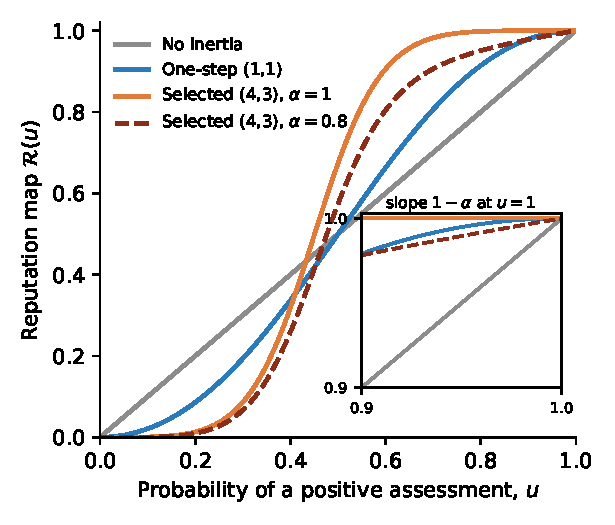
\includegraphics[width=\linewidth,height=0.84\textheight,keepaspectratio]{reputation_map}\par}
\vspace{3pt}\figcap{$\mathscr{R}(u)$ for SJ architectures. Inset: near $u=1$ the slope is $1-\alpha$.}
\end{column}
\end{columns}
\end{frame}

% ---------------------------------------------------------------- slide 20
\begin{frame}{From single records to population reputations}\relax
{\small \textbf{Mean-field closure.} (A1) Donor and observer images of a recipient are independent given its strategy. (A2) Assessments entering a record are independent with probability $u_I$.\par}\vspace{3pt}
\eqline{\small}{u_{\mathrm{ALLC}}=\Phi_{\mathrm{C}}(\bar r),\quad u_{\mathrm{ALLD}}=\Phi_{\mathrm{D}}(\bar r),\quad u_{\mathrm{DISC}}=h_{\mathrm{GG}}P^{+}_{\mathrm{C|G}}+h_{\mathrm{GB}}\bigl(P^{+}_{\mathrm{C|B}}+P^{+}_{\mathrm{D|G}}\bigr)+h_{\mathrm{BB}}P^{+}_{\mathrm{D|B}}}
\eqlead{Self-consistency, with the branch reached from initially good records:}
\eqline{\small}{r_I^*=\mathscr{R}\bigl(u_I(\boldsymbol{r}^*;\boldsymbol{f})\bigr),\qquad \frac{\mathrm{d}r_I}{\mathrm{d}\tau}=\mathscr{R}(u_I)-r_I,\quad r_I(0)=1}
\eqlead{Homogeneous DISC population:}
\eqline{\small}{u_{\mathrm{R}}(r)=r\,\Phi_{\mathrm{C}}(r)+(1-r)\,\Phi_{\mathrm{D}}(r),\qquad F(r)=\mathscr{R}\bigl[u_{\mathrm{R}}(r)\bigr]-r}
{\small Stable roots have $F'<0$, and folds satisfy $F=F'=0$. The resident reputation $r_{\mathrm{R}}^*$ is the highest strictly stable root.\par}\vspace{3pt}
\end{frame}

% ---------------------------------------------------------------- slide 21
\begin{frame}{Strategy evolution and measures of cooperation}\relax
\eqlead{Payoffs per unit time, with stationary reputations recomputed at every composition:}
\eqline{\small}{\Pi_I=(1-e_1)\bigl[b\,(f_{\mathrm{ALLC}}+f_{\mathrm{DISC}}\,r_I^*)-c\,\chi_I\bigr],\qquad \chi_{\mathrm{ALLC}}=1,\ \chi_{\mathrm{ALLD}}=0,\ \chi_{\mathrm{DISC}}=\bar r^*}
\eqlead{Replicator dynamics and cooperation:}
\eqline{\small}{\dot f_I=f_I\bigl(\Pi_I-\bar\Pi\bigr),\qquad \bar\rho\approx\omega_{\mathrm{C}}\,\bar\rho_{\mathrm{C}}}
{\small
\begin{itemize}
  \item Intended cooperation $\rho_{\mathrm{int}}=f_{\mathrm{ALLC}}+f_{\mathrm{DISC}}\,\bar r^*$; realized $\rho=(1-e_1)\rho_{\mathrm{int}}\leq0.98$.
  \item $\bar\rho$: mean long-run cooperation over 512 area-uniform initial compositions; $\omega_{\mathrm{C}}$: cooperative basin; $\bar\rho_{\mathrm{C}}$: cooperation within it.
\end{itemize}}
\end{frame}

% ---------------------------------------------------------------- slide 22
\begin{frame}{Local stability against rare unconditional mutants}\relax
\eqlead{A rare mutant X that intends to help with probability $\chi_{\mathrm{X}}$ (ALLD: $\chi=0$, ALLC: $\chi=1$):}
\eqline{\small}{\Lambda_{\mathrm{X}}=\frac{\Pi_{\mathrm{X}}-\Pi_{\mathrm{R}}}{c(1-e_1)}=\bigl(r_{\mathrm{R}}^*-\chi_{\mathrm{X}}\bigr)-\frac{b}{c}\bigl(r_{\mathrm{R}}^*-r_{\mathrm{X}}^*\bigr),\qquad r_{\mathrm{X}}^*=\mathscr{R}(u_{\mathrm{X}})}
\eqlead{Pure DISC resists both ALLD and ALLC if and only if}
\eqline{\small}{R_{\mathrm{L}}=\frac{r_{\mathrm{R}}^*}{r_{\mathrm{R}}^*-\mathscr{R}(\Phi^*_{\mathrm{D}})}<\frac{b}{c}<\frac{1-r_{\mathrm{R}}^*}{\mathscr{R}(\Phi^*_{\mathrm{C}})-r_{\mathrm{R}}^*}=R_{\mathrm{U}}}
\eqlead{The window is open if and only if $\mathscr{R}$ lies above its chord:}
\eqline{\small}{R_{\mathrm{L}}<R_{\mathrm{U}}\iff r_{\mathrm{R}}^*\,\mathscr{R}(\Phi^*_{\mathrm{C}})+(1-r_{\mathrm{R}}^*)\,\mathscr{R}(\Phi^*_{\mathrm{D}})<\mathscr{R}(u_{\mathrm{R}}^*)}
\takeaway{Without inertia $\mathscr{R}$ is linear, so no $b/c$ protects pure DISC. Inertia bends $\mathscr{R}$ and opens the window.}
\end{frame}

% ---------------------------------------------------------------- slide 23
\begin{frame}{Opportunistic discriminators (O-DISC)}\relax
{\small O-DISC withholds help from a recipient it regards as good with probability $\delta$ ($\delta=0$: DISC, $\delta=1$: ALLD).\par}\vspace{3pt}
\eqline{\small}{\Lambda(\delta)=\delta\,r_{\mathrm{R}}^*-\frac{b}{c}\bigl[r_{\mathrm{R}}^*-r_{\mathrm{X}}^*(\delta)\bigr],\qquad u_{\mathrm{X}}(\delta)=u_{\mathrm{R}}^*-\delta\,r_{\mathrm{R}}^*\,\Delta\Phi^*}
\eqlead{Weak opportunism invades when the reputation response is flat:}
\eqline{\small}{\Lambda'(0)=r_{\mathrm{R}}^*\Bigl[1-\frac{b}{c}\,\Delta\Phi^*\,\mathscr{R}'(u_{\mathrm{R}}^*)\Bigr]}
\eqlead{Every O-DISC mutant is excluded if and only if}
\eqline{\small}{H_{\min}=\min_{0\leq\delta\leq1}\frac{r_{\mathrm{R}}^*-r_{\mathrm{X}}^*(\delta)}{\delta\,r_{\mathrm{R}}^*}\geq\frac{c}{b}}
\begin{alertblock}{Exact result in the error-free limit}
{\small $e_1=e_2=0$, $\beta=1$, $k_1\geq1$: every O-DISC mutant is excluded if and only if $\alpha\leq1-c/b$ (i.e. $\alpha\leq0.8$ at $b/c=5$), for all four norms and all $k_2$.\par}
\end{alertblock}
\end{frame}

% ---------------------------------------------------------------- slide 24
\section{Results}
{\setbeamercolor{background canvas}{bg=ink}
\begin{frame}[plain,noframenumbering]
\vspace*{2.0cm}
{\color{accent}\fontsize{40}{44}\selectfont\bfseries 3\par}
\vspace{0.3cm}
{\color{white}\fontsize{22}{26}\selectfont\bfseries Results\par}
\end{frame}}

% ---------------------------------------------------------------- slide 25
\begin{frame}{Directional inertia restores recognition and agreement}\relax
\begin{columns}[T,onlytextwidth]
\begin{column}{0.63\textwidth}
{\centering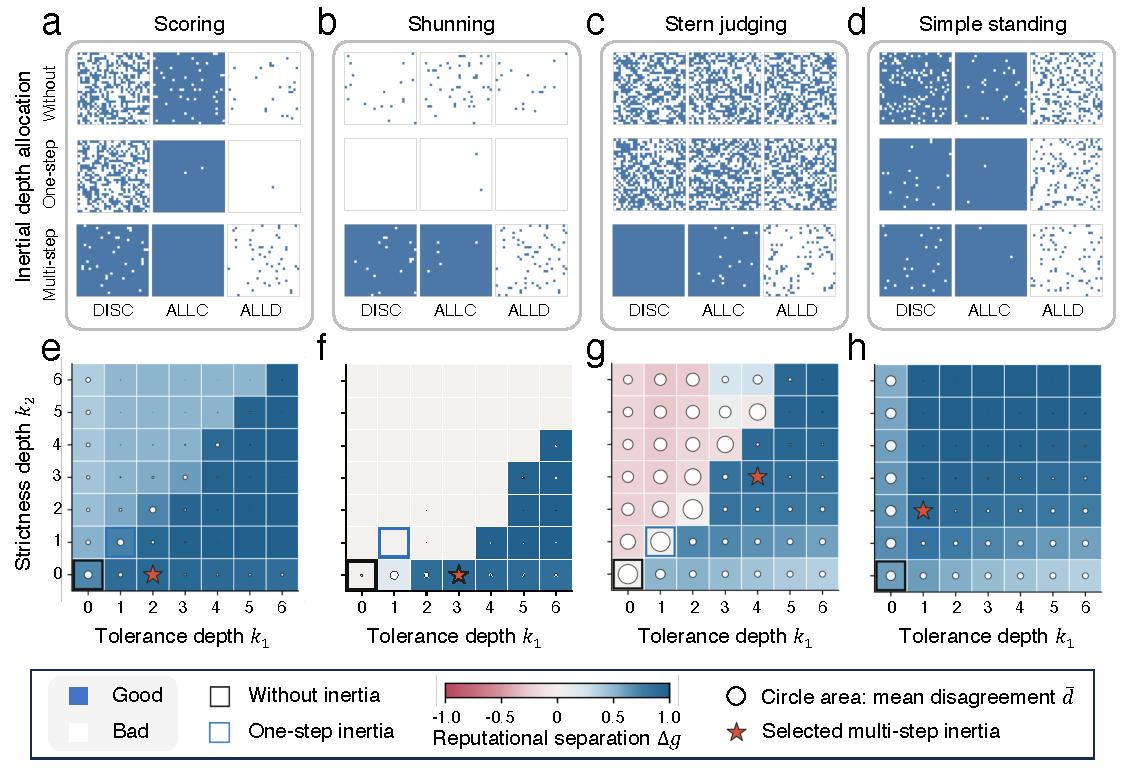
\includegraphics[width=\linewidth,height=0.82\textheight,keepaspectratio]{Fig2}\par}
\end{column}
\hfill
\begin{column}{0.34\textwidth}
\figcap{\textbf{Fig. 2} | \textbf{a–d}, private image matrices (rows: DISC observers; columns: DISC, ALLC, ALLD targets; blue: good) without inertia, with one-step inertia and with the selected architectures. \textbf{e–h}, separation $\Delta g$ (color) and disagreement $\bar d$ (circle area) across $k_1$, $k_2$. Stars: smallest $K$ with $\Delta g\geq0.8$ and $\bar d\leq0.1$.}
\vspace{4pt}
\takeaway{One-step inertia fails: SH agrees that everyone is bad, and SJ keeps disagreeing. Norm-specific allocations achieve both recognition and agreement.}
\end{column}
\end{columns}
\end{frame}

% ---------------------------------------------------------------- slide 26
\begin{frame}{Selected architectures make cooperation stable and accessible}\relax
\begin{columns}[T,onlytextwidth]
\begin{column}{0.63\textwidth}
{\centering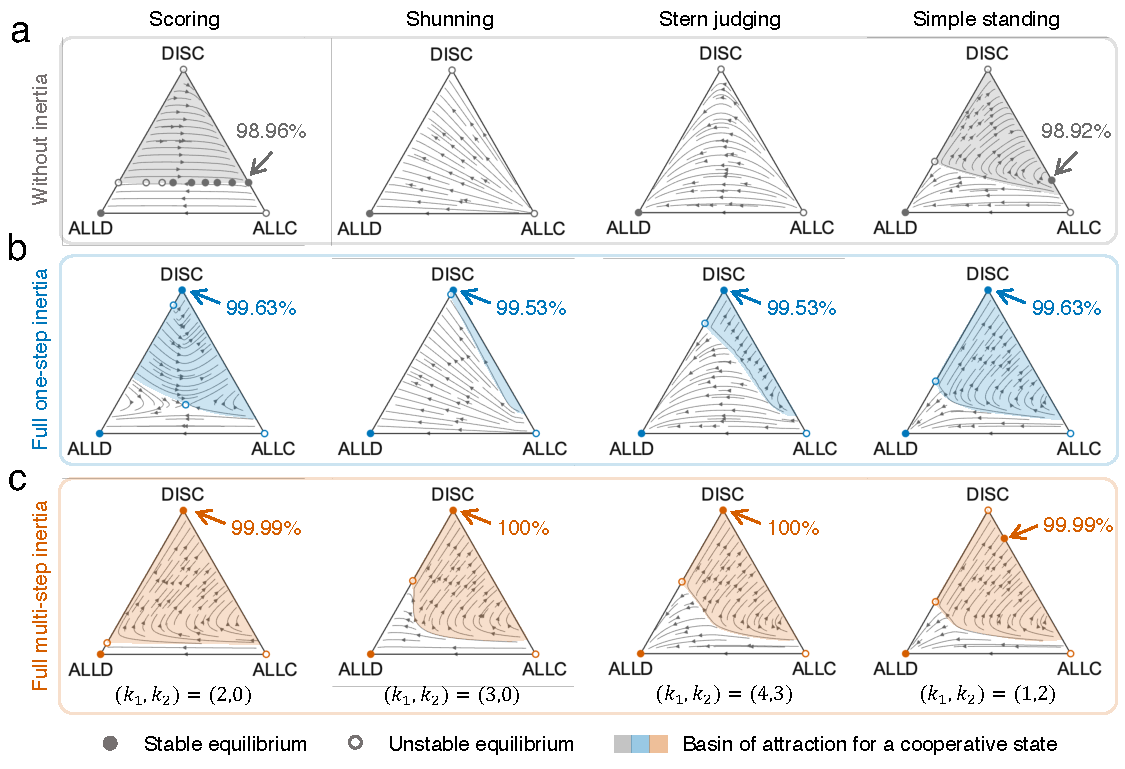
\includegraphics[width=\linewidth,height=0.82\textheight,keepaspectratio]{Fig3}\par}
\end{column}
\hfill
\begin{column}{0.34\textwidth}
\figcap{\textbf{Fig. 3} | Replicator dynamics of ALLC, ALLD and DISC without inertia (\textbf{a}), with one-step inertia (\textbf{b}) and with the selected architectures (\textbf{c}). Filled and open circles: stable and unstable equilibria. Shading: basin of a cooperative state. Percentages: intended cooperation. $b/c=5$, $e_1=e_2=0.02$.}
\vspace{4pt}
\takeaway{Cooperative basins grow from 8\% (SH) and 23\% (SJ) under one-step inertia to 70–88\% under the selected architectures. Under SS, the attractor is a stable DISC–ALLC mixture.}
\vspace{2pt}\smallnote{SC panel in \textbf{a} to be redrawn as a single line of equilibria.}
\end{column}
\end{columns}
\end{frame}

% ---------------------------------------------------------------- slide 27
\begin{frame}{Allocation, not amount, determines cooperation}\relax
\begin{columns}[T,onlytextwidth]
\begin{column}{0.63\textwidth}
{\centering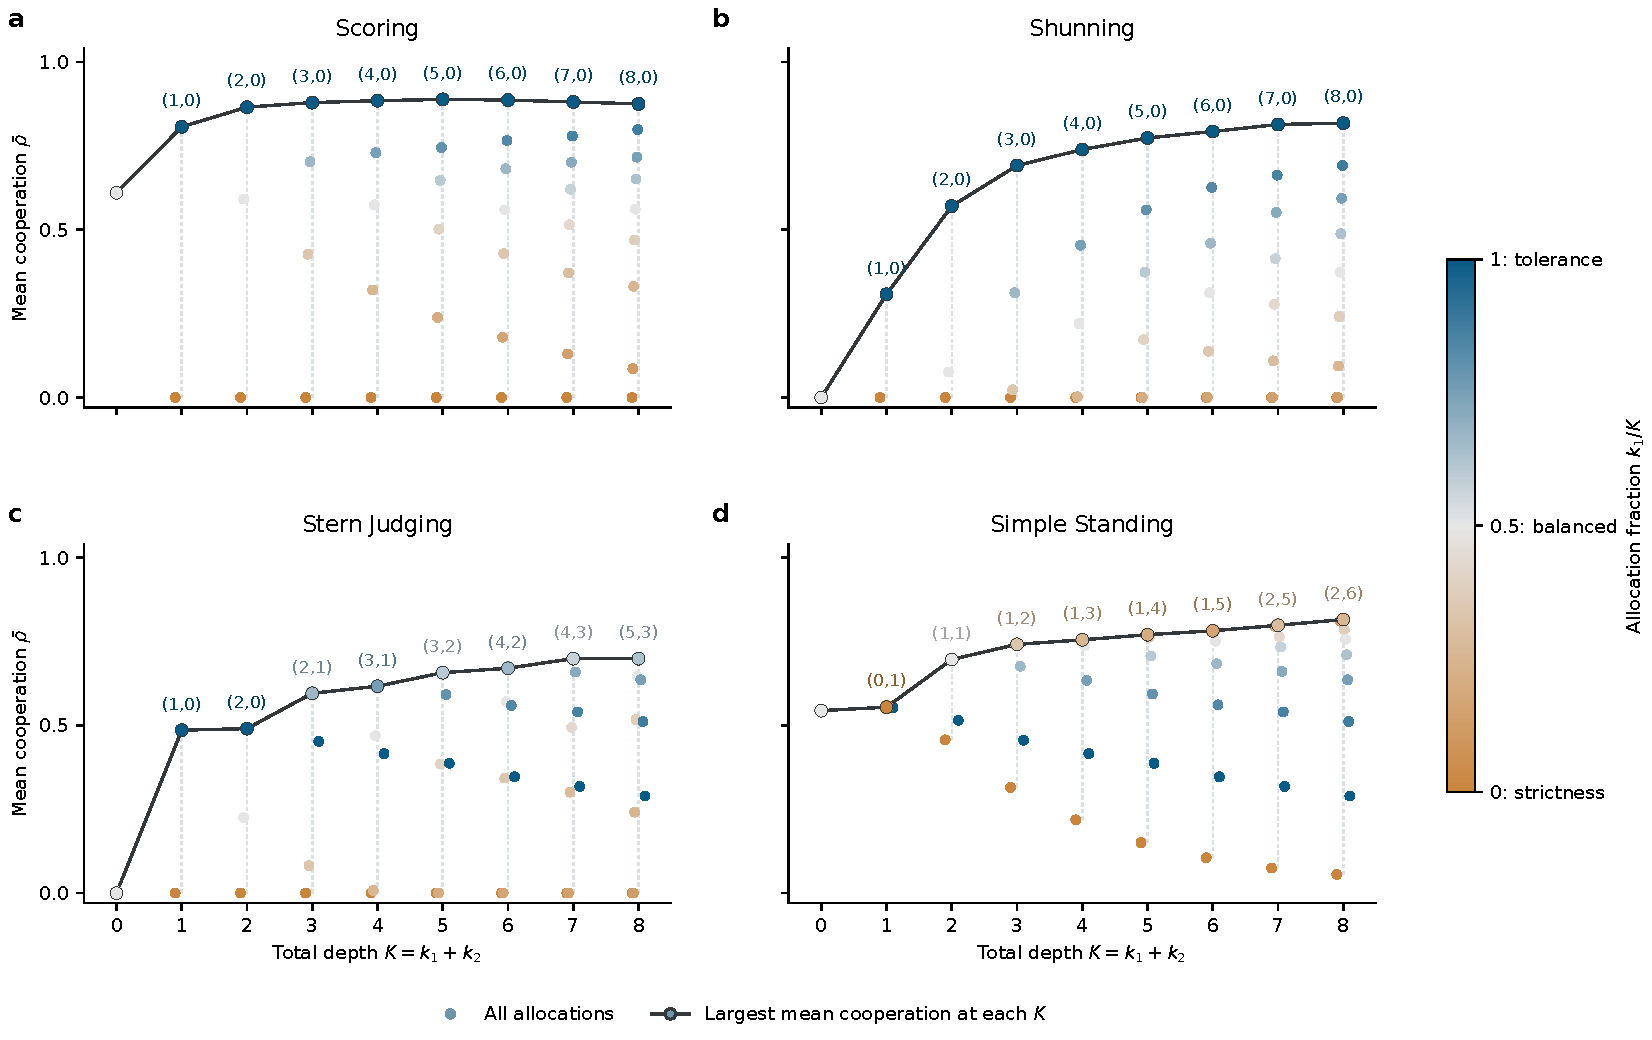
\includegraphics[width=\linewidth,height=0.82\textheight,keepaspectratio]{Fig4_verified}\par}
\end{column}
\hfill
\begin{column}{0.34\textwidth}
\figcap{\textbf{Fig. 4} | Mean realized cooperation $\bar\rho$ (512 initial compositions) for every allocation $(k_1,k_2)$ at total depth $K$. Color: tolerance fraction $k_1/K$. Black line: best allocation at each $K$. $\alpha=\beta=1$, $b/c=5$.}
\vspace{4pt}
\takeaway{At fixed depth, cooperation ranges from none to high depending on direction. The reputation-selected architectures are the best allocations at their depths, and extra depth saturates.}
\vspace{2pt}\smallnote{Rendered from the verified data; manuscript artwork to be updated.}
\end{column}
\end{columns}
\end{frame}

% ---------------------------------------------------------------- slide 28
\begin{frame}{Tolerance invites opportunism; lower tolerance strength restores deterrence}\relax
{\centering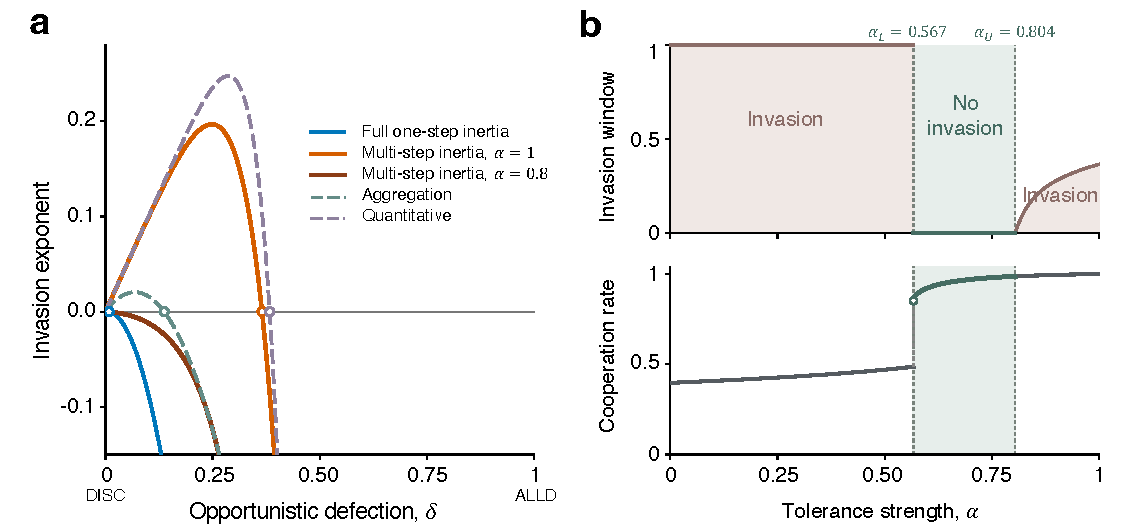
\includegraphics[width=\linewidth,height=0.49\textheight,keepaspectratio]{Fig5}\par}
\vspace{3pt}
\figcap{\textbf{Fig. 5} | \textbf{a}, invasion payoff $\Lambda(\delta)$ of O-DISC under SJ: one-step inertia, $(4,3)$ with $\alpha=1$ and $0.8$, aggregation and a quantitative score. \textbf{b}, $(4,3)$ against $\alpha$: invasion endpoint $\delta_c$ (top) and resident cooperation (bottom). Green: secure range $\alpha_{\mathrm{L}}<\alpha\leq\alpha_{\mathrm{U}}$. $\beta=1$, $b/c=5$.}
\takeaway{All mechanisms exclude ALLD, yet partial opportunists invade ($0<\delta<0.365$ for $(4,3)$ at $\alpha=1$). For $0.57<\alpha\leq0.80$, every O-DISC mutant is excluded and cooperation stays high.}
\end{frame}

% ---------------------------------------------------------------- slide 29
\section{Conclusion}
{\setbeamercolor{background canvas}{bg=ink}
\begin{frame}[plain,noframenumbering]
\vspace*{2.0cm}
{\color{accent}\fontsize{40}{44}\selectfont\bfseries 4\par}
\vspace{0.3cm}
{\color{white}\fontsize{22}{26}\selectfont\bfseries Conclusion\par}
\end{frame}}

% ---------------------------------------------------------------- slide 30
\begin{frame}{Back to the research gap}\relax
\vspace{4pt}\begin{tabular}{@{}>{\raggedright\arraybackslash}p{0.31\linewidth}>{\raggedright\arraybackslash}p{0.64\linewidth}@{}}
\toprule
{\small\bfseries\color{blueacc}How should reputations integrate evidence over time?} & {\small Separately for losing and regaining standing. The \textbf{allocation} of inertia, not its amount, decides whether private reputations are accurate and shared.} \\
\midrule
{\small\bfseries\color{blueacc}Does this matter for the evolution of cooperation?} & {\small Yes. Compact architectures selected on reputational criteria alone make cooperation \textbf{stable and accessible} under all four norms.} \\
\midrule
{\small\bfseries\color{blueacc}Is tolerance safe?} & {\small No. Tolerance \textbf{shelters occasional defectors} even when ALLD is excluded. Partial consequences of warning states ($\alpha<1$) restore deterrence while cooperation stays high.} \\
\bottomrule
\end{tabular}
\end{frame}

% ---------------------------------------------------------------- slide 31
{\setbeamercolor{background canvas}{bg=ink}
\begin{frame}[plain,noframenumbering]
\vspace*{1.3cm}
\begin{center}
\begin{minipage}{0.86\textwidth}
{\color{white}\fontsize{17}{23}\selectfont\bfseries Reputation-based cooperation depends not only on which behaviors are judged good, but also on how reputations accumulate and express behavioral evidence.\par}
\end{minipage}

\vspace{1.0cm}
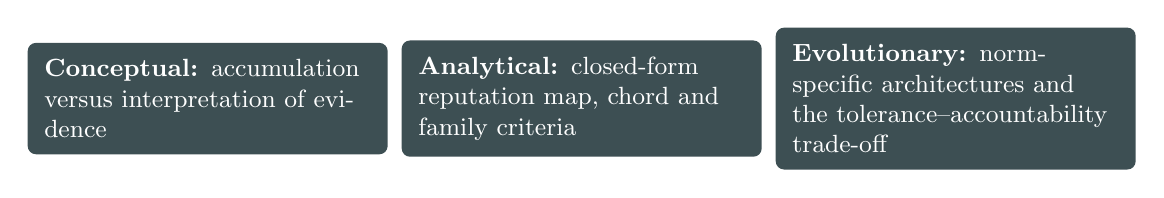
\begin{tikzpicture}
  \node[fill=white!12!ink,rounded corners=3pt,text width=4.15cm,minimum height=1.25cm,align=left,font=\small,text=white,inner sep=6pt] at (0.00,0) {\textbf{Conceptual:} accumulation versus interpretation of evidence};
  \node[fill=white!12!ink,rounded corners=3pt,text width=4.15cm,minimum height=1.25cm,align=left,font=\small,text=white,inner sep=6pt] at (4.75,0) {\textbf{Analytical:} closed-form reputation map, chord and family criteria};
  \node[fill=white!12!ink,rounded corners=3pt,text width=4.15cm,minimum height=1.25cm,align=left,font=\small,text=white,inner sep=6pt] at (9.50,0) {\textbf{Evolutionary:} norm-specific architectures and the tolerance–accountability trade-off};
\end{tikzpicture}
\end{center}
\end{frame}}

% ---------------------------------------------------------------- slide 32
\begin{frame}{Points for discussion}\relax
\begin{columns}[T,onlytextwidth]
\begin{column}{0.313\textwidth}
\begin{block}{Narrative and venue}
\begin{cardlist}
  \item Storyline A or B?
  \item Target journal and framing
\end{cardlist}
\end{block}
\end{column}
\hfill
\begin{column}{0.313\textwidth}
\begin{block}{Evolving architectures}
\begin{cardlist}
  \item Let $k_1$, $k_2$, $\alpha$, $\beta$ evolve
  \item Co-evolution with norms
\end{cardlist}
\end{block}
\end{column}
\hfill
\begin{column}{0.313\textwidth}
\begin{block}{Strategic opportunism}
\begin{cardlist}
  \item Defections timed to the record
  \item Temporally correlated omissions
\end{cardlist}
\end{block}
\end{column}
\end{columns}
\vspace{4pt}
\begin{columns}[T,onlytextwidth]
\begin{column}{0.313\textwidth}
\begin{block}{Beyond mean field}
\begin{cardlist}
  \item Simultaneous reputation and strategy change
  \item Structured populations
\end{cardlist}
\end{block}
\end{column}
\hfill
\begin{column}{0.313\textwidth}
\begin{block}{Combining mechanisms}
\begin{cardlist}
  \item Inertia plus opinion synchronization
  \item Dual (recipient) assessment
\end{cardlist}
\end{block}
\end{column}
\hfill
\begin{column}{0.313\textwidth}
\begin{block}{Empirical tests}
\begin{cardlist}
  \item Partial distrust after a single lapse
  \item Norm-dependent asymmetric updating
\end{cardlist}
\end{block}
\end{column}
\end{columns}
\vspace{4pt}
\end{frame}

% ---------------------------------------------------------------- slide 33
\appendix
\section{Supplementary results}
{\setbeamercolor{background canvas}{bg=ink}
\begin{frame}[plain,noframenumbering]
\vspace*{2.0cm}
{\color{accent}\fontsize{40}{44}\selectfont\bfseries 5\par}
\vspace{0.3cm}
{\color{white}\fontsize{22}{26}\selectfont\bfseries Supplementary results\par}
\end{frame}}

% ---------------------------------------------------------------- slide 34
\begin{frame}{Selection is robust across criteria}\relax
\begin{columns}[T,onlytextwidth]
\begin{column}{0.63\textwidth}
{\centering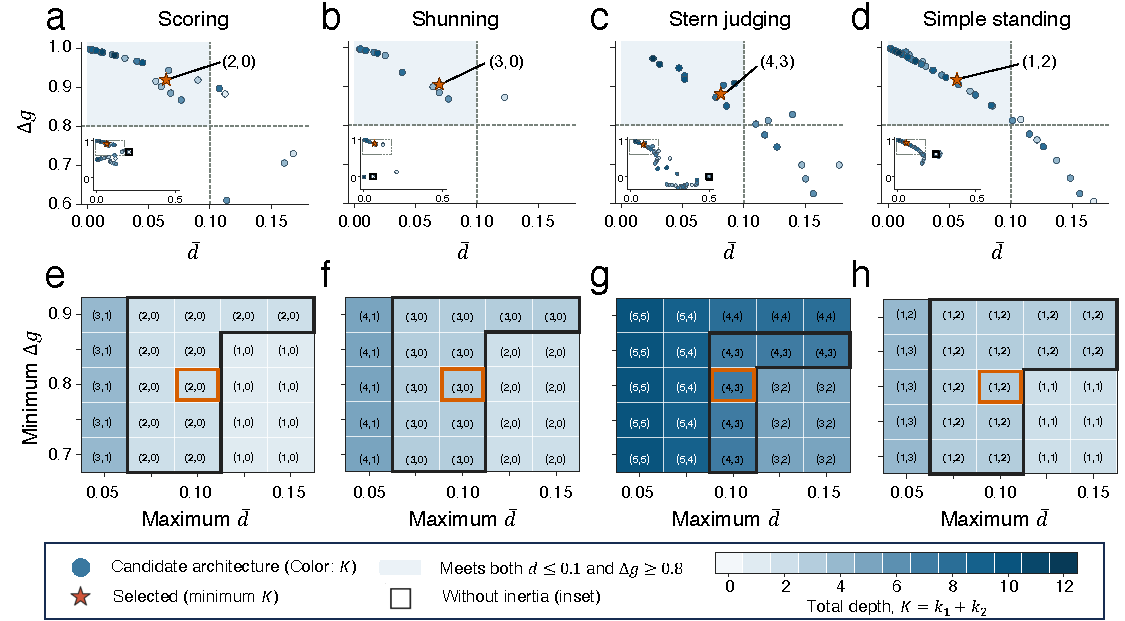
\includegraphics[width=\linewidth,height=0.82\textheight,keepaspectratio]{ED_Fig1}\par}
\end{column}
\hfill
\begin{column}{0.34\textwidth}
\figcap{\textbf{Extended Data Fig. 1} | \textbf{a–d}, $\Delta g$ against $\bar d$ for all depth pairs (30 replicates; color: total depth $K$); stars: selected pairs. \textbf{e–h}, minimum-depth pair selected as the separation and disagreement thresholds vary; orange: default criteria.}
\vspace{4pt}
\takeaway{Exact depth pairs depend on the thresholds, but compact, norm-specific architectures qualify over a wide range of criteria.}
\end{column}
\end{columns}
\end{frame}

% ---------------------------------------------------------------- slide 35
\begin{frame}{One-step inertia is bistable; the selected architectures are not}\relax
\begin{columns}[T,onlytextwidth]
\begin{column}{0.63\textwidth}
{\centering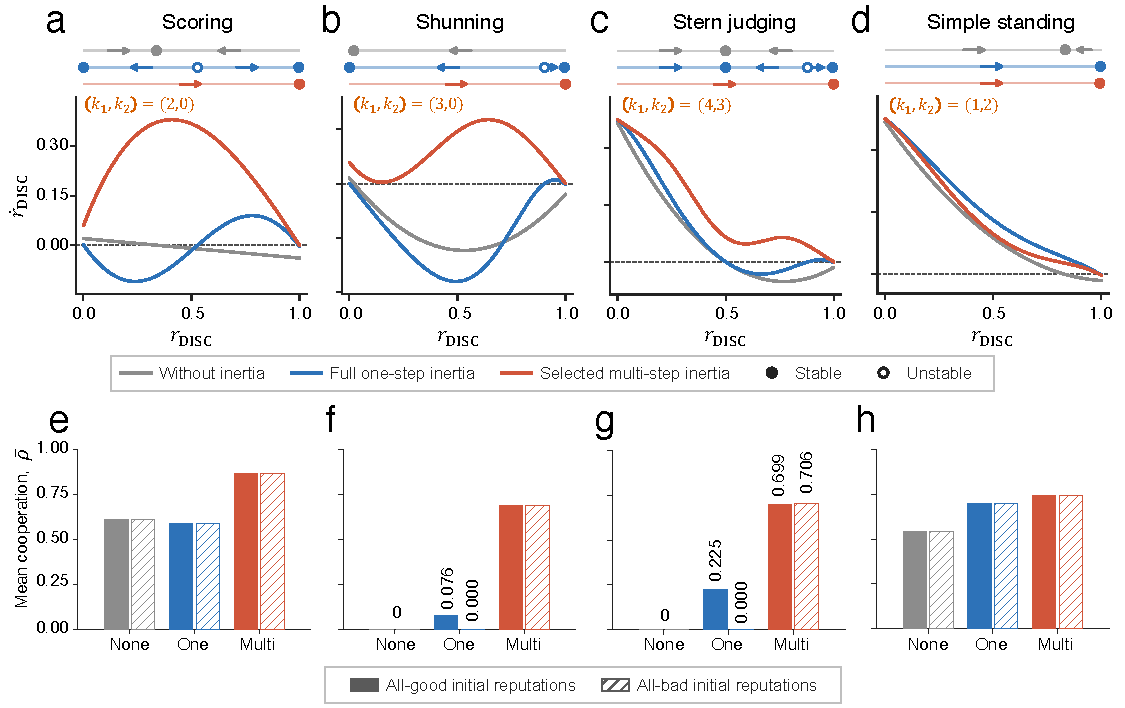
\includegraphics[width=\linewidth,height=0.82\textheight,keepaspectratio]{ED_Fig2}\par}
\end{column}
\hfill
\begin{column}{0.34\textwidth}
\figcap{\textbf{Extended Data Fig. 2} | \textbf{a–d}, reputation dynamics in homogeneous DISC populations (gray: none; blue: one-step; red: selected). \textbf{e–h}, mean cooperation $\bar\rho$ after all-good (solid) and all-bad (hatched) initial reputations.}
\vspace{4pt}
\takeaway{One-step inertia leaves SC, SH and SJ bistable, so cooperation under SH and SJ collapses from all-bad records. The selected architectures have a single high-reputation state.}
\end{column}
\end{columns}
\end{frame}

% ---------------------------------------------------------------- slide 36
\begin{frame}{Strengths and depths jointly shape reputation equilibria}\relax
\begin{columns}[T,onlytextwidth]
\begin{column}{0.63\textwidth}
{\centering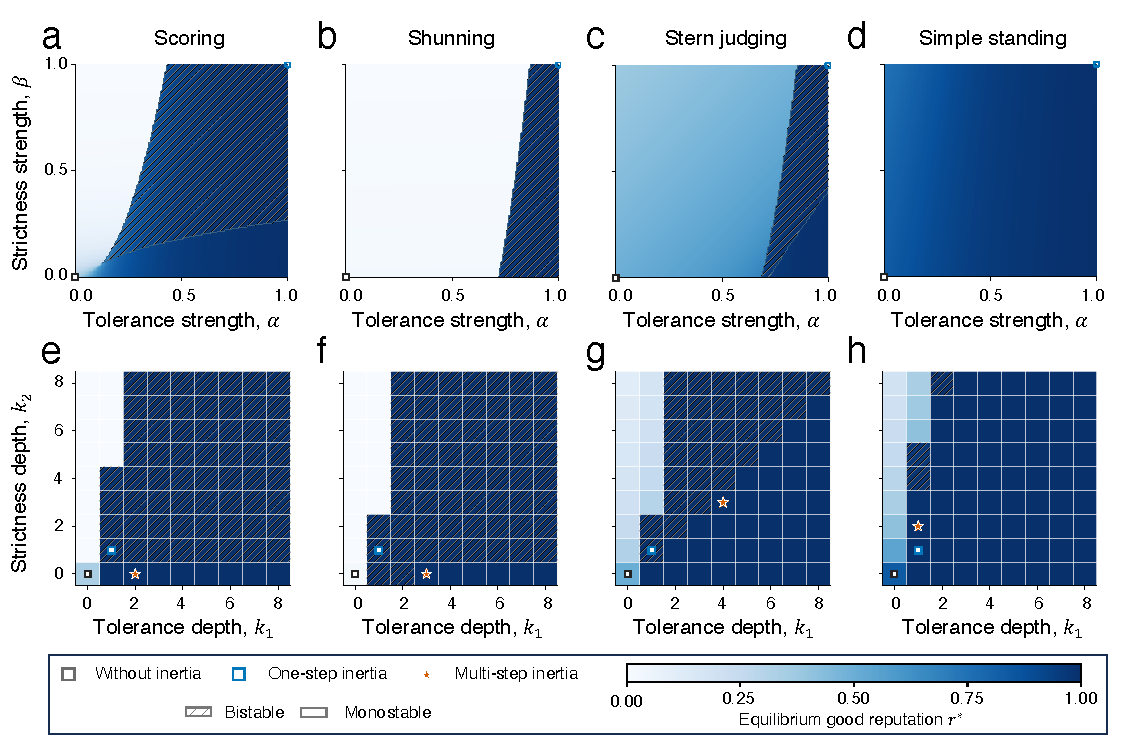
\includegraphics[width=\linewidth,height=0.82\textheight,keepaspectratio]{ED_Fig3}\par}
\end{column}
\hfill
\begin{column}{0.34\textwidth}
\figcap{\textbf{Extended Data Fig. 3} | Highest stable reputation of a homogeneous DISC population across $(\alpha,\beta)$ at one-step depths (\textbf{a–d}) and across $(k_1,k_2)$ with $\alpha=\beta=1$ (\textbf{e–h}). Hatching: bistability; stars: selected architectures.}
\vspace{4pt}
\takeaway{Reputation levels and bistability depend on the norm and on the direction and strength of inertia.}
\end{column}
\end{columns}
\end{frame}

% ---------------------------------------------------------------- slide 37
\begin{frame}{Why basins expand: the ALLD–DISC edge}\relax
\begin{columns}[T,onlytextwidth]
\begin{column}{0.63\textwidth}
{\centering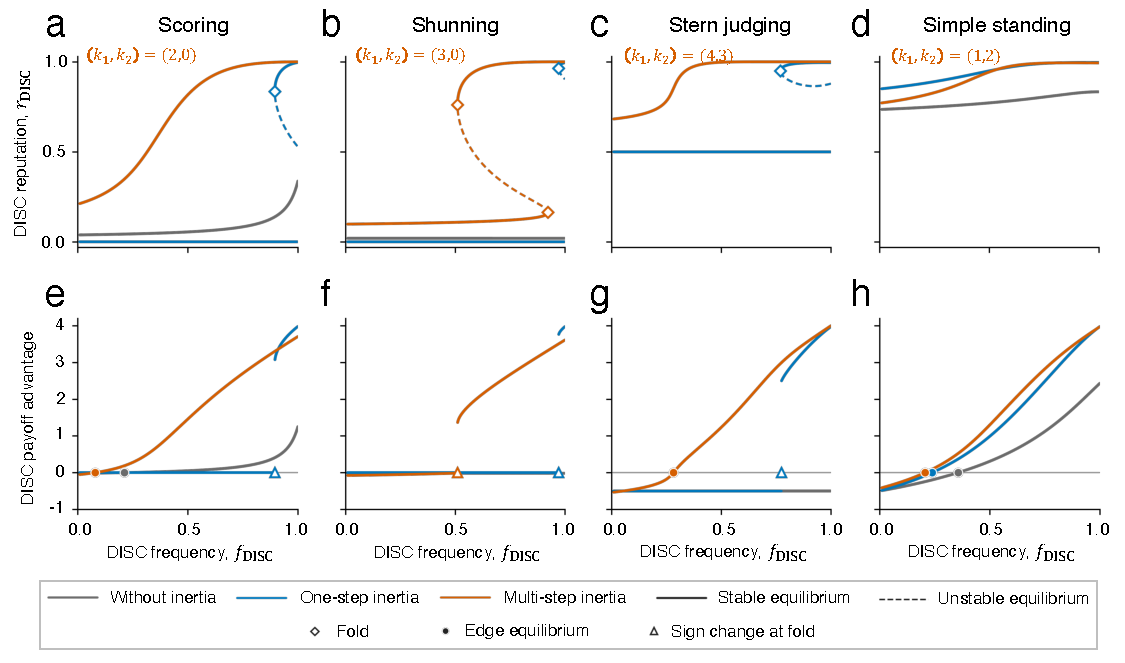
\includegraphics[width=\linewidth,height=0.82\textheight,keepaspectratio]{ED_Fig4}\par}
\end{column}
\hfill
\begin{column}{0.34\textwidth}
\figcap{\textbf{Extended Data Fig. 4} | \textbf{a–d}, DISC reputation along the ALLD–DISC edge (solid: stable; dashed: unstable; diamonds: folds). \textbf{e–h}, payoff advantage of DISC over ALLD on the all-good branch.}
\vspace{4pt}
\takeaway{Under one-step inertia DISC loses its good reputation abruptly when rare. The selected architectures shift (SH) or remove (SC, SJ) this fold.}
\end{column}
\end{columns}
\end{frame}

% ---------------------------------------------------------------- slide 38
\begin{frame}{Benefit-to-cost ratio and local protection}\relax
\begin{columns}[T,onlytextwidth]
\begin{column}{0.63\textwidth}
{\centering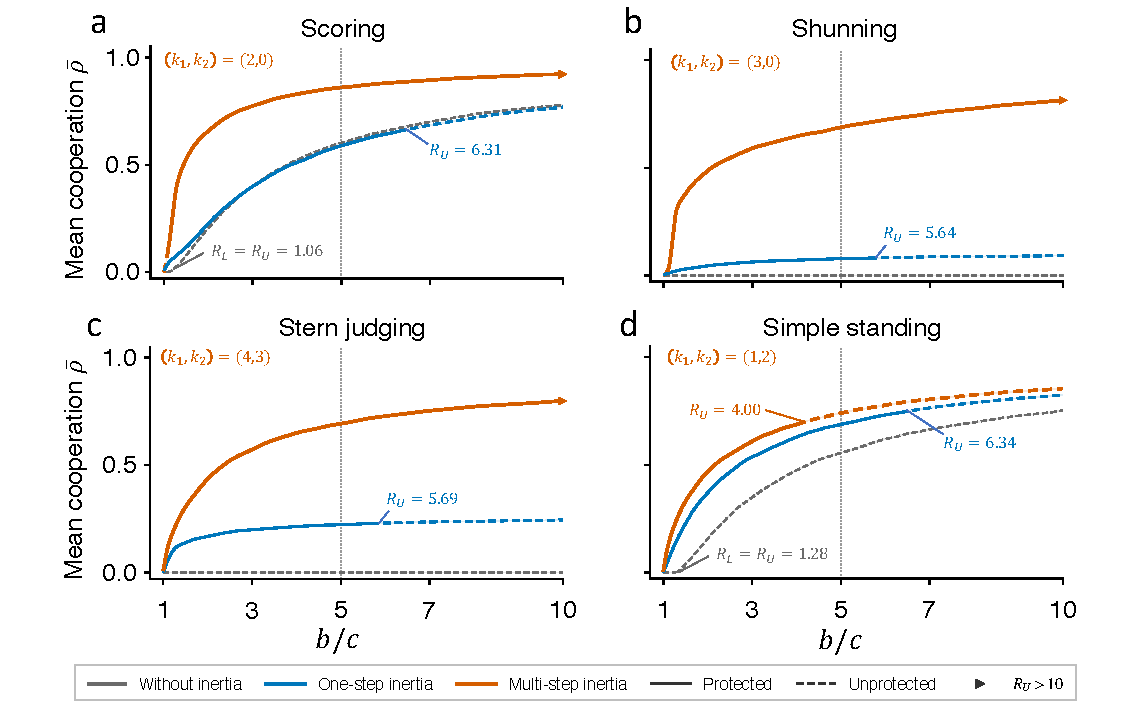
\includegraphics[width=\linewidth,height=0.82\textheight,keepaspectratio]{ED_Fig5}\par}
\end{column}
\hfill
\begin{column}{0.34\textwidth}
\figcap{\textbf{Extended Data Fig. 5} | Mean cooperation $\bar\rho$ against $b/c$. Solid: pure DISC resists ALLC and ALLD ($R_{\mathrm{L}}<b/c<R_{\mathrm{U}}$); dashed: not protected. Means over eight samples of 512 initial compositions.}
\vspace{4pt}
\takeaway{The selected architectures give the most cooperation across $b/c$. Under SS, cooperation stays high even above $R_{\mathrm{U}}\approx4$.}
\end{column}
\end{columns}
\end{frame}

% ---------------------------------------------------------------- slide 39
\begin{frame}{Tolerance and strictness strengths act differently}\relax
\begin{columns}[T,onlytextwidth]
\begin{column}{0.63\textwidth}
{\centering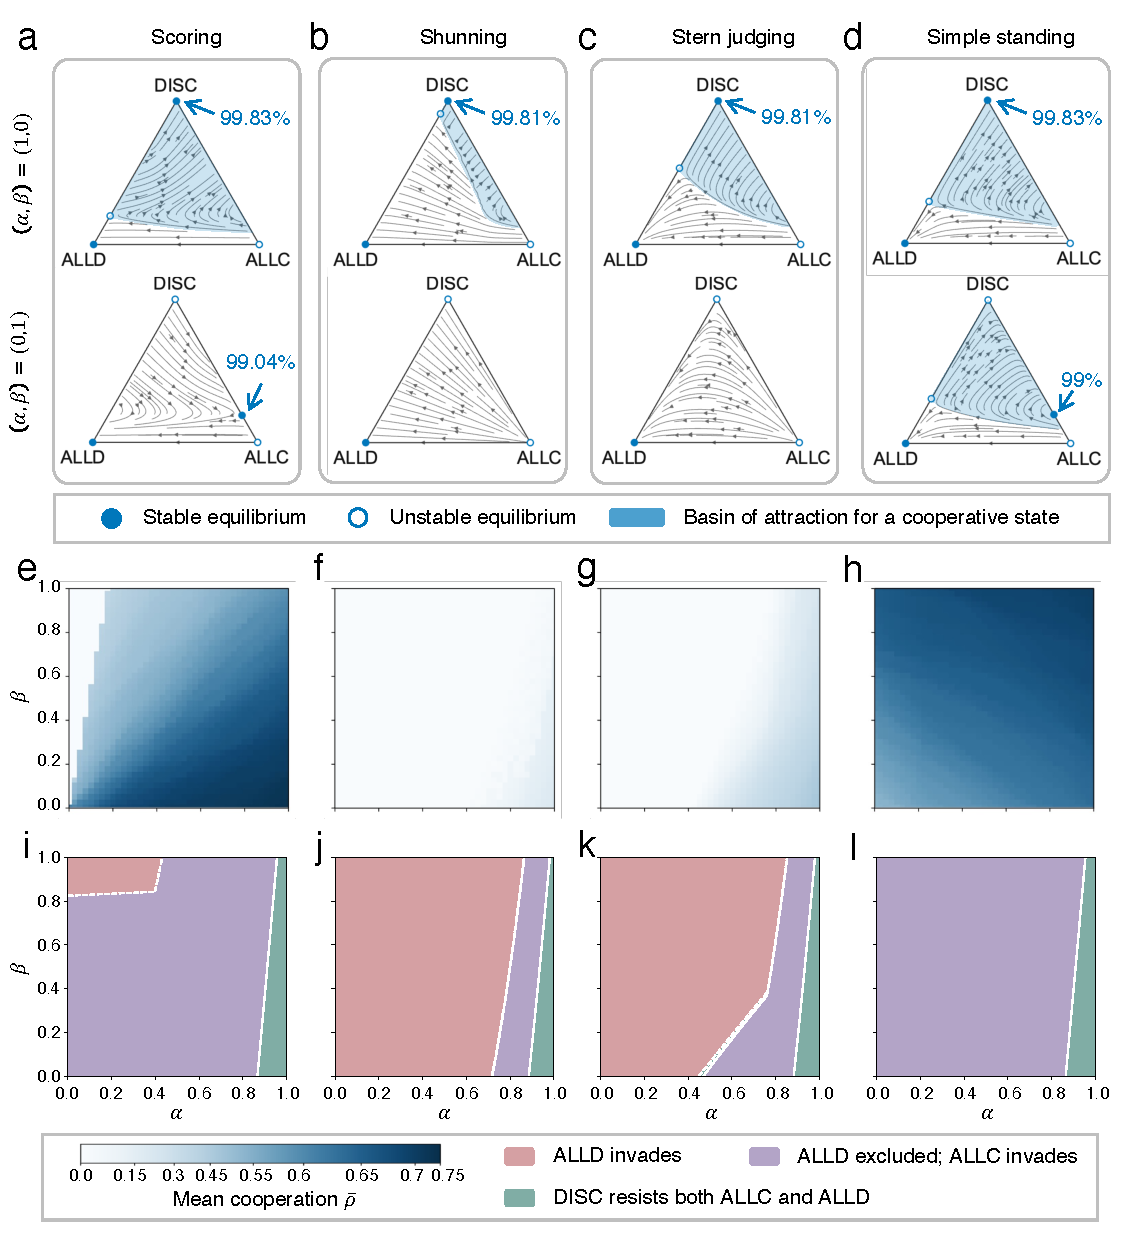
\includegraphics[width=\linewidth,height=0.82\textheight,keepaspectratio]{ED_Fig6}\par}
\end{column}
\hfill
\begin{column}{0.34\textwidth}
\figcap{\textbf{Extended Data Fig. 6} | One-step depths. \textbf{a–d}, dynamics with tolerance only, $(\alpha,\beta)=(1,0)$ (top), and strictness only, $(0,1)$ (bottom). \textbf{e–h}, mean cooperation over the $(\alpha,\beta)$ plane. \textbf{i–l}, local invasion classes.}
\vspace{4pt}
\takeaway{Tolerance only stabilizes highly cooperative DISC populations under all four norms. Strictness only does not, and its effect depends on the norm.}
\end{column}
\end{columns}
\end{frame}

% ---------------------------------------------------------------- slide 40
\begin{frame}{Local protection across error rates}\relax
\begin{columns}[T,onlytextwidth]
\begin{column}{0.63\textwidth}
{\centering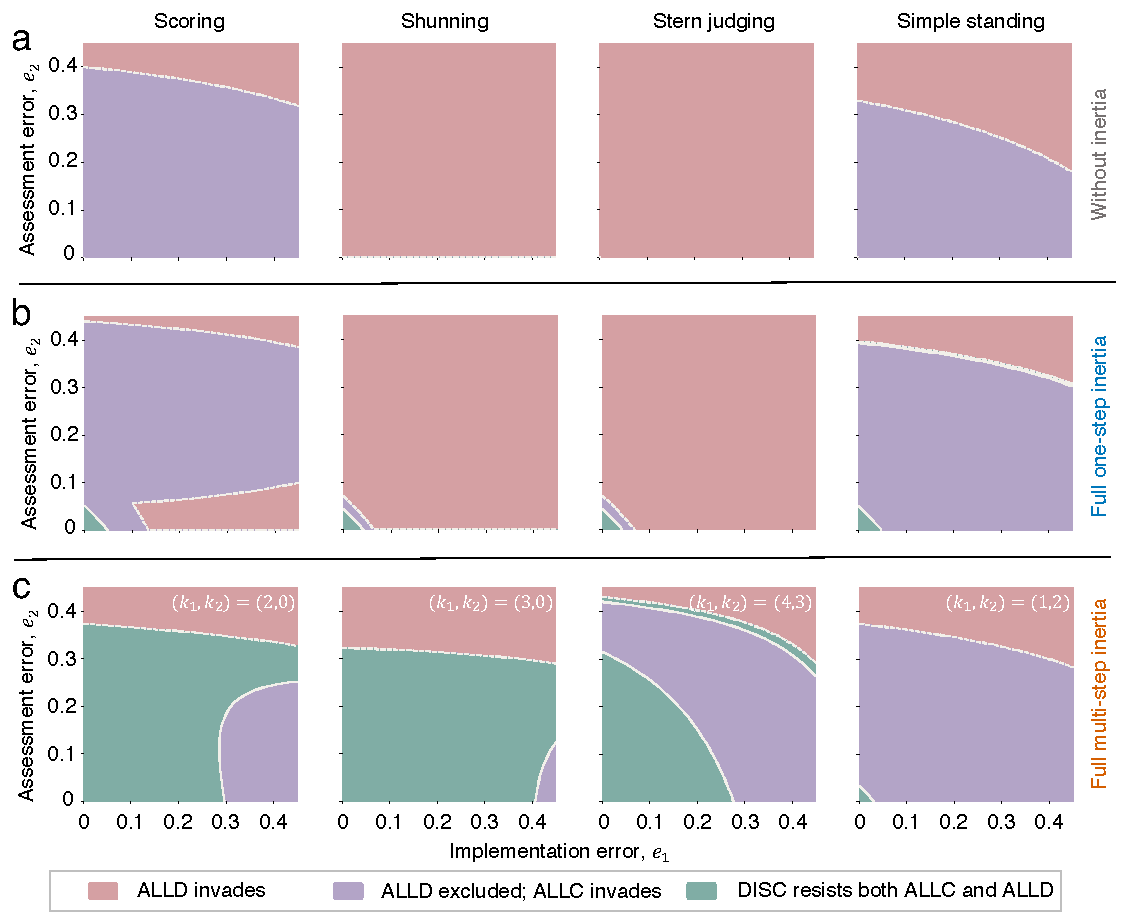
\includegraphics[width=\linewidth,height=0.82\textheight,keepaspectratio]{ED_Fig7}\par}
\end{column}
\hfill
\begin{column}{0.34\textwidth}
\figcap{\textbf{Extended Data Fig. 7} | Local invasion classes over implementation error $e_1$ and assessment error $e_2$ without inertia (\textbf{a}), with one-step inertia (\textbf{b}) and with the selected architectures (\textbf{c}). Pink: ALLD invades; purple: ALLC invades; green: DISC resists both.}
\vspace{4pt}
\takeaway{The selected architectures exclude ALLD over most error rates under SH and SJ, and protect DISC against both mutants over most of the plane under SC and SH.}
\end{column}
\end{columns}
\end{frame}

% ---------------------------------------------------------------- slide 41
\begin{frame}{Cooperation and protection across the depth plane}\relax
{\centering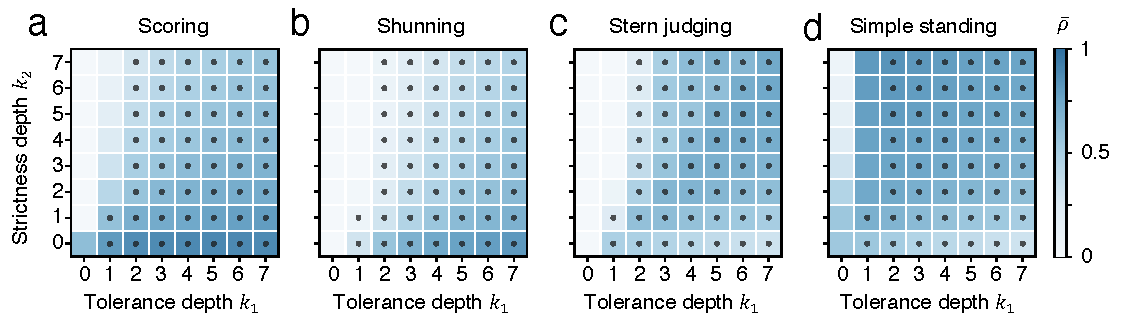
\includegraphics[width=\linewidth,height=0.49\textheight,keepaspectratio]{ED_Fig8}\par}
\vspace{3pt}
\figcap{\textbf{Extended Data Fig. 8} | Mean cooperation $\bar\rho$ over $(k_1,k_2)$; dots: pure DISC resists rare ALLC and ALLD. $\alpha=\beta=1$, $b/c=5$.}
\takeaway{High cooperation follows norm-specific directions, and local protection of pure DISC does not coincide with high population-level cooperation.}
\end{frame}

% ---------------------------------------------------------------- slide 42
\begin{frame}{Secure tolerance strengths across norms and benefit-to-cost ratios}\relax
\begin{columns}[T,onlytextwidth]
\begin{column}{0.63\textwidth}
{\centering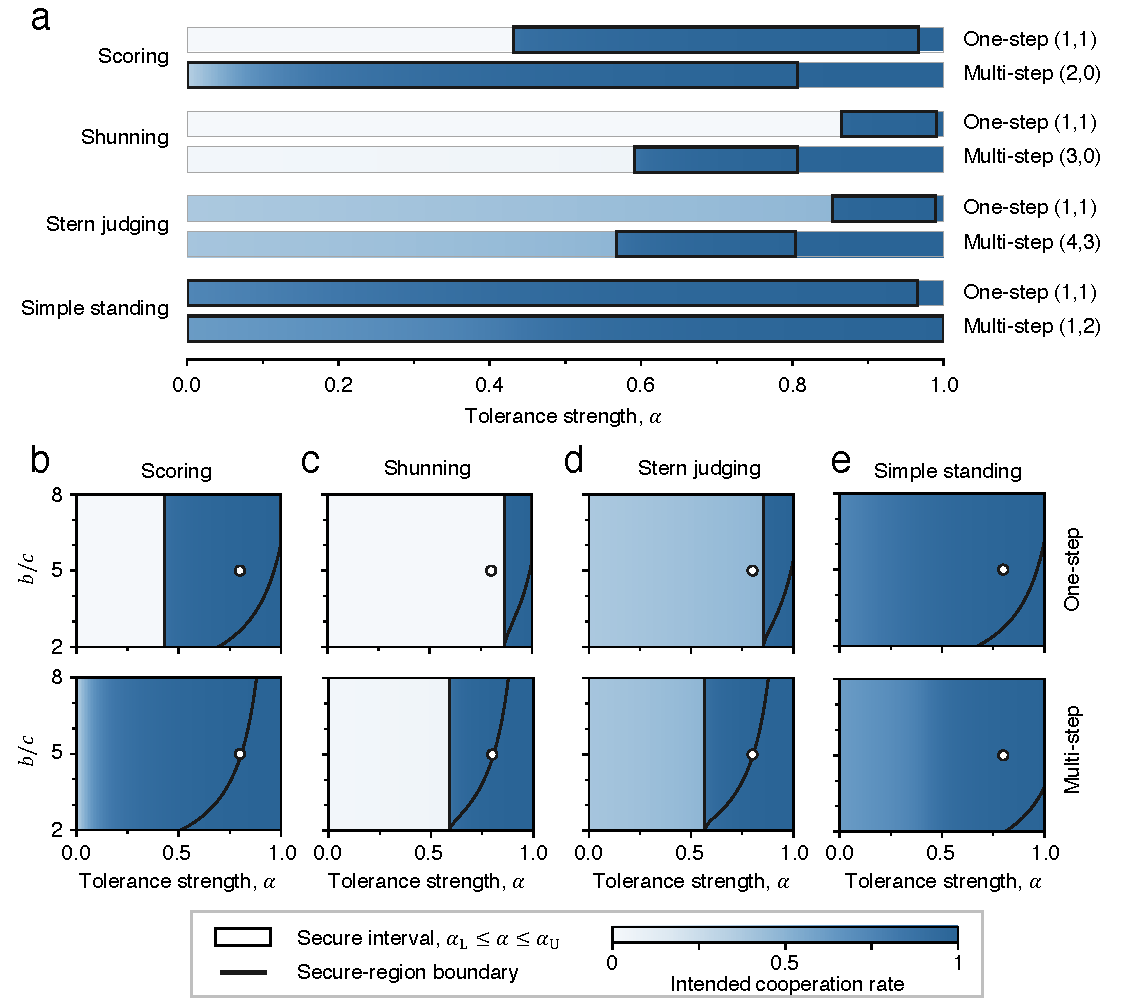
\includegraphics[width=\linewidth,height=0.82\textheight,keepaspectratio]{ED_Fig9}\par}
\end{column}
\hfill
\begin{column}{0.34\textwidth}
\figcap{\textbf{Extended Data Fig. 9} | \textbf{a}, secure intervals of $\alpha$ at $b/c=5$ for one-step and selected architectures (black frames; shading: resident cooperation). \textbf{b–e}, security across $\alpha$ and $b/c$; circles: $(\alpha,b/c)=(0.8,5)$.}
\vspace{4pt}
\takeaway{At $\alpha=0.8$ all selected architectures resist O-DISC with high cooperation. Protective ranges shrink as $b/c$ decreases and close under SH at $b/c=2$.}
\end{column}
\end{columns}
\end{frame}

% ---------------------------------------------------------------- slide 43
\begin{frame}{Analytical highlights}\relax
{\small
\begin{tabular}{@{}>{\raggedright\arraybackslash}p{\dimexpr0.240\linewidth-2\tabcolsep\relax}>{\raggedright\arraybackslash}p{\dimexpr0.760\linewidth-2\tabcolsep\relax}@{}}
\toprule
\rowcolor{cardbg}\textbf{Result} & \textbf{Statement} \\
\midrule
\textbf{No window without inertia} & If $\mathscr{R}(u)=u$, then $R_{\mathrm{L}}=R_{\mathrm{U}}=1/\Delta\Phi^*$, so no $b/c$ protects pure DISC against both ALLD and ALLC. \\
\textbf{Chord condition} & The protection window is open if and only if $\mathscr{R}$ lies above its chord between $\Phi^*_{\mathrm{D}}$ and $\Phi^*_{\mathrm{C}}$ at $u_{\mathrm{R}}^*$. \\
\textbf{Worst opportunist} & If $\mathscr{R}$ is concave (e.g. $k_2=0$), $H$ is non-decreasing in $\delta$, so $\Lambda'(0)\leq0$ excludes the whole O-DISC family. \\
\textbf{Error-free threshold} & With $\beta=1$ and $k_1\geq1$, an all-good resident excludes every O-DISC mutant if and only if $\alpha\leq1-c/b$. \\
\textbf{Closing of secure intervals} & Near a fold the interval closes at $b/c=u_{\mathrm{R}}'/\Delta\Phi$, which equals 2 under SH for all errors and depths. \\
\textbf{SC without inertia} & A line of equilibria at $f_{\mathrm{DISC}}=c/[b(\varepsilon-e_2)]$, attracting on the ALLC side and repelling on the ALLD side. \\
\bottomrule
\end{tabular}}\par\vspace{3pt}
\end{frame}

% ---------------------------------------------------------------- slide 44
\begin{frame}{Reference values}\relax
\begin{columns}[T,onlytextwidth]
\begin{column}{0.44\textwidth}
{\small \textbf{Local protection thresholds} ($\alpha=\beta=1$)\par}\vspace{3pt}
{\footnotesize
\begin{tabular}{@{}>{\raggedright\arraybackslash}p{\dimexpr0.150\linewidth-2\tabcolsep\relax}>{\raggedright\arraybackslash}p{\dimexpr0.370\linewidth-2\tabcolsep\relax}>{\raggedright\arraybackslash}p{\dimexpr0.230\linewidth-2\tabcolsep\relax}>{\raggedright\arraybackslash}p{\dimexpr0.230\linewidth-2\tabcolsep\relax}@{}}
\toprule
\rowcolor{cardbg}\textbf{Norm} & \textbf{Setting} & \textbf{$r_{\mathrm{R}}^*$} & \textbf{$R_{\mathrm{U}}$} \\
\midrule
\textbf{SC} & one-step & 0.9963 & 6.31 \\
 & selected (2,0) & 0.9999 & 230 \\
\textbf{SH} & one-step & 0.9953 & 5.64 \\
 & selected (3,0) & 1.0000 & 4410 \\
\textbf{SJ} & one-step & 0.9953 & 5.69 \\
 & selected (4,3) & 1.0000 & 20910 \\
\textbf{SS} & one-step & 0.9963 & 6.34 \\
 & selected (1,2) & 0.9937 & 4.00 \\
\bottomrule
\end{tabular}}\par\vspace{3pt}
{\small {\color{muted}$R_{\mathrm{L}}$ lies between 1.00 and 1.08 in all inertial cases.}\par}\vspace{3pt}
\end{column}
\hfill
\begin{column}{0.52\textwidth}
{\small \textbf{Basin $\omega_{\mathrm{C}}$ and mean cooperation $\bar\rho$}\par}\vspace{3pt}
{\footnotesize
\begin{tabular}{@{}>{\raggedright\arraybackslash}p{\dimexpr0.130\linewidth-2\tabcolsep\relax}>{\raggedright\arraybackslash}p{\dimexpr0.290\linewidth-2\tabcolsep\relax}>{\raggedright\arraybackslash}p{\dimexpr0.290\linewidth-2\tabcolsep\relax}>{\raggedright\arraybackslash}p{\dimexpr0.290\linewidth-2\tabcolsep\relax}@{}}
\toprule
\rowcolor{cardbg}\textbf{Norm} & \textbf{None} & \textbf{One-step} & \textbf{Selected} \\
\midrule
\textbf{SC} & 0.63 / 0.61 & 0.61 / 0.59 & 0.88 / 0.87 \\
\textbf{SH} & 0 / 0 & 0.08 / 0.08 & 0.71 / 0.69 \\
\textbf{SJ} & 0 / 0 & 0.23 / 0.22 & 0.71 / 0.70 \\
\textbf{SS} & 0.56 / 0.54 & 0.71 / 0.70 & 0.76 / 0.74 \\
\bottomrule
\end{tabular}}\par\vspace{3pt}
{\small {\color{muted}512 initial compositions, $b/c=5$.}\par}\vspace{3pt}
\end{column}
\end{columns}
\end{frame}

% ---------------------------------------------------------------- slide 45
\begin{frame}[allowframebreaks]{References}
\nocite{milinski2016,nowak1998,nowak2005,ohtsuki2004,ohtsuki2006,hilbe2018,fujimoto2022,fujimoto2023,radzvilavicius2019,okada2020,radzvilavicius2021,kawakatsu2024,murase2023,murase2024synchronization,tham2026,schmid2021,schmid2023,clark2020,michelmata2024,yamamoto2025,ostrom1990,cox2010,tadelis2016,blumstein2009,mendesiedlecki2013neural,mendesiedlecki2013diagnostic,slovic1993,siegel2018}
\tiny
\bibliographystyle{plainnat}
\bibliography{slides_refs}
\end{frame}

\end{document}
